\documentclass{article}
\usepackage{a4wide}


\usepackage{polski}
\usepackage[utf8x]{inputenc}
\usepackage{graphicx}
\usepackage{float}
\usepackage{hyperref}
\usepackage{listings}
\usepackage{mathtools}
\usepackage{amsmath}
\usepackage{hyperref}
\usepackage[margin=1in]{geometry}

\author{Lev Sergeyev}
\title{ZAPDC \\ Ćwiczenie 3 \\ Zastosowania interpolacji - demozaikowanie}

\date{ }
\begin{document}

\maketitle

%\pagebreakmovie15

\section{Przebieg ćwiczenia}
Zaprojektowałem dwie funkcje, które pozwalają na mozaikowanie/demozaikowanie obrazu o zadany filtr CFA(korzystałem z filtrów Bayer'a i X-Trans).  \\
\par
\textbf{Funkcja mozaikowania.} Filtruje obraz zadaną macierz filtru, przy czym pobrany obraz o 3 kanałach jest zapisywany do obrazu(macierzy) 1-kanałowego. \\
\par
\textbf{Funkcja demozaikowania.} Na podstawie macierzy filtru funkcja odtwarza obraz po mozaikowaniu, dla każdego nowego piksela pobierając informację o pikselach z okna 2x2, liczy średnią ważoną(waga brana jest z macierzy filtru). W praktyce demozaikowanie używa \textbf{interpolację funkcją liniową}, gdzie punkt interpolowany leży w \( P( \frac{x_2 - x_1}{2} , \frac{y_2 - y_1}{2} ) \). \\
Dodatkowo zaprojektowałem rozszerzoną wersję funkcji demozaikowania, w której można zadać rozmiar okna i kroku.

\section{Porównywanie otrzymanych obrazów}

\subsection{Bayer}
\begin{center}
    \begin{tabular}{ | p{3cm} | c |}
    \hline
    Operacja &  Obraz \\ \hline
    
    \smallskip mozaikowanie & 
    \raisebox{-\totalheight}{\scalebox{0.5}{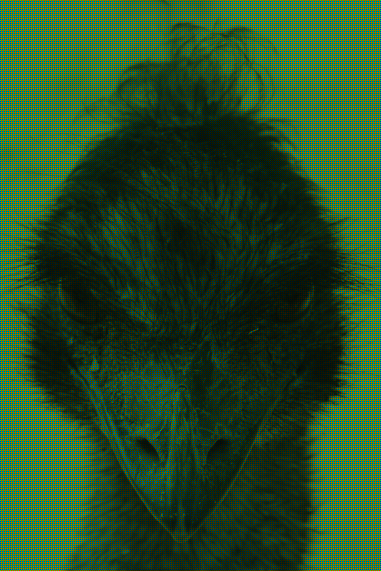
\includegraphics{img/bayer_mos.png}}}
     \\ \hline

    \smallskip demozaikowanie  & 
    \raisebox{-\totalheight}{\scalebox{0.5}{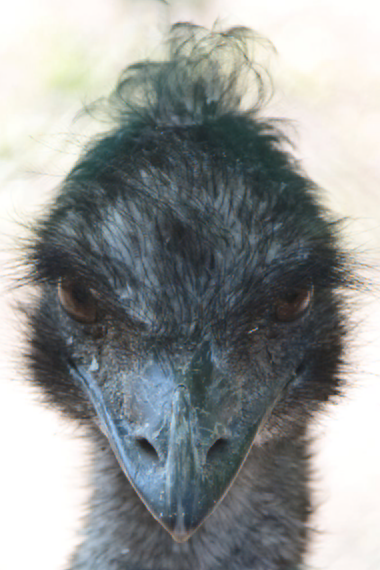
\includegraphics{img/bayer_dmos.png}}} 
    \\ \hline
    \end{tabular}
\end{center}

\pagebreak

\subsection{X-Trans}
\begin{center}
    \begin{tabular}{ | p{3cm} | c |}
    \hline
    Operacja &  Obraz \\ \hline
    
    \smallskip mozaikowanie & 
    \raisebox{-\totalheight}{\scalebox{0.45}{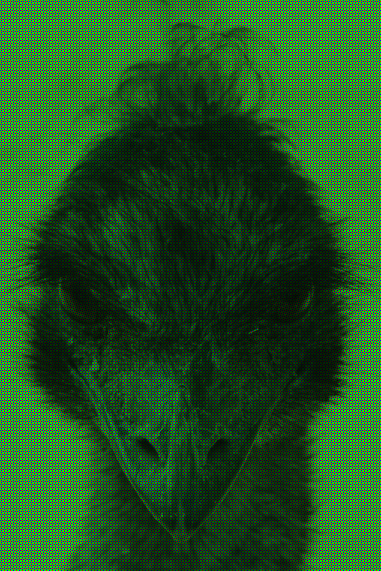
\includegraphics{img/xtrans_mos.png}}}
     \\ \hline

    \smallskip demozaikowanie  & 
    \raisebox{-\totalheight}{\scalebox{0.45}{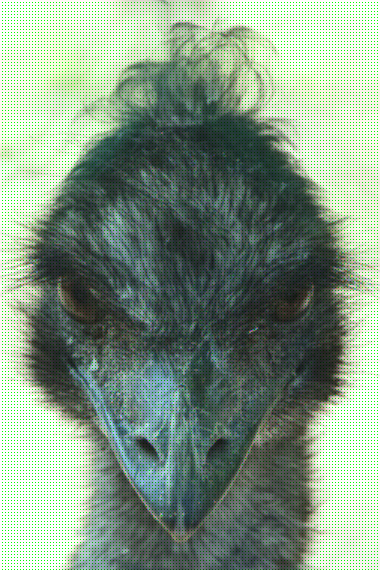
\includegraphics{img/xtrans_dmos.png}}} 
    \\ \hline
    
    \smallskip demozaikowanie, okno: 3x3, krok:1x1 (domyślny) & 
    \raisebox{-\totalheight}{\scalebox{0.45}{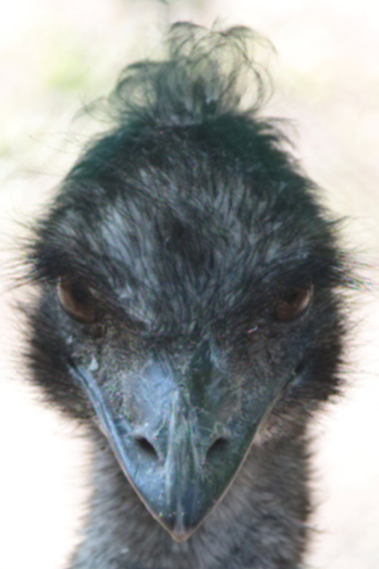
\includegraphics{img/xtrans_dmos_adv_w3.png}}} 
    \\ \hline
    \end{tabular}
\end{center}

\subsection{Kod}
\href{https://github.com/221349/ZAPDC/tree/master/lab6}{https://github.com/221349/ZAPDC/tree/master/lab6}

\section{Wnioski}
\par
Jednym z najprostrzych i szybszych metod demozaikowania jest zastosowanie interplolacji. \\
Algorytm z zastosowaniem interpolacji dwuliniowej dobrze radzi z demozaikowaniem obrazu po filtracji CFA Bayer. \\
W przypadku mozaiki X-Trans, przez strukturę filtru, algorytm demozaikowania z oknem 2x2 powoduje powstanie "zielonych" pikseli z krokiem 3x3, w tym przypadku można zastosować demozaikowanie z oknem większym niż 2x2.
\par 
Demozaikowanie interpolacją należy do najprostrzych metod demozaikowania, zaletą jest niska złożoność algorytmu, przez co często jest wbudowane w matrycę CCD lub CMOS. \\
Wadą można nazwać mniej dokładny obraz po demozaikowaniu(szczególnie przy większym oknie i kroku) w porównaniu do bardziej zaawansowanych metod demozaikowania.


\end{document}
